\authoredsubsection{Sprint 2}{Gáspár}{Gáspár Harmati}\label{sec:sprint2}

Sprint 2 ran from 12 to 25 May 2026, with the review and retrospective on 26 May. Sprint 1 had produced the scientific and architectural foundation; this sprint translated it into the first working code. Gáspár Harmati took the Scrum Master role.

\subsubsection{Sprint Goals}\label{sec:sprint2-goals}

The sprint goal was that the chatbot application routes queries to eight specialized agents using initial system prompts, that traces are persisted to a database, that a first synthetic dataset is available in the pipeline repository, and that the judge and the prompt optimizer are implemented and connected to the router. The goal was specific in naming each component, measurable in that each either exists in the repository or does not, and time-bound to the two-week sprint \autocite{schwaber2020scrum}.

\subsubsection{Sprint Planning}\label{sec:sprint2-planning}

Seven tickets totaling 25 story points were planned, consistent with the velocity of Sprint 1: the eight agents and their system prompts and the batch-evaluation wiring with Sebastian Straub, the synthetic dataset with Gáspár Harmati, the agent prompt design with Mohsin Saeed, the multi-agent dispatcher and trace database with Julius Bethge, the judge with Marco Schröder, and the optimizer MVP with Gáspár Harmati and Mohsin Saeed jointly. Responding to Sprint 1 feedback, the team added a fixed in-person working session on Tuesdays ahead of the weekly Interhyp check-in and kept two online stand-ups per week.

\subsubsection{Implementation and Execution}\label{sec:sprint2-execution}

The eight-agent roster for the real estate brokerage scenario was defined in this sprint, with the eighth slot filled by a PropertyLawAgent and only later settled in favor of the PlatformSupportAgent for the reasons set out in \cref{sec:agent-architecture}. The first synthetic dataset was generated and calibrated against an internal Interhyp frequency reference, with the tail imbalance deliberately softened so that rarely called agents still receive enough samples to be scored (\cref{sec:dataset-stages}). Each agent prompt was given the same five-part structure of role, task, constraints, output format, and quality check, so that the router had clearer boundaries between agents with overlapping responsibilities.

The dispatcher was built as the two-stage architecture that the router still uses today: a cheap embedding stage, at this point on BAAI/bge-small-en-v1.5 with a single global threshold, followed by a log-probability stage on a locally served Gemma 4 model. Every call was written to a trace database behind a FastAPI backend, with a React cockpit visualizing the pipeline. The judge was implemented as a panel of independent models, following the finding that a panel of smaller models outperforms a single large judge at lower cost \autocite{verga2024juries,li_llms-as-judges_2024}; the panel was reduced to a single judge later in the project (\cref{sec:judge-bias}). The optimizer MVP implemented OPRO \autocite{yang2023llmoptimizers} against a mocked judge, so that both modules could be developed in parallel, and it still rewrote the judge prompt rather than the routing prompt it targets in the final system (\cref{sec:optimizer}).

\subsubsection{Sprint Review}\label{sec:sprint2-review}

Julian Kappler represented Interhyp at the review on 26 May, as Rainer Bomblies was unavailable. He confirmed that the domain analogy and the dataset calibration were a sufficiently close match to Interhyp's setup, and asked for a dashboard presenting routing accuracy against the secondary KPIs as a single accuracy-performance frontier, so that the effect of a prompt change could be read off directly. He also cautioned against scope creep, arguing that a smaller set of components finished with measurable results would be worth more than a larger partially working system, and asked the team to log the full candidate ranking per trace rather than only the selected agent.

All 25 story points were delivered, but the burndown shows the same late-finishing pattern as Sprint 1 (\cref{fig:sprint2-burndown}): the small tickets closed early while the three five-point tickets finished in the last days. The cumulative flow diagram (\cref{fig:sprint2-cumulative-flow}) shows the same effect from the other side, with a steady band of in-progress work through the sprint. The spike on 26 May is backlog grooming for Sprint 3 rather than Sprint 2 work.

\begin{figure}
\centering
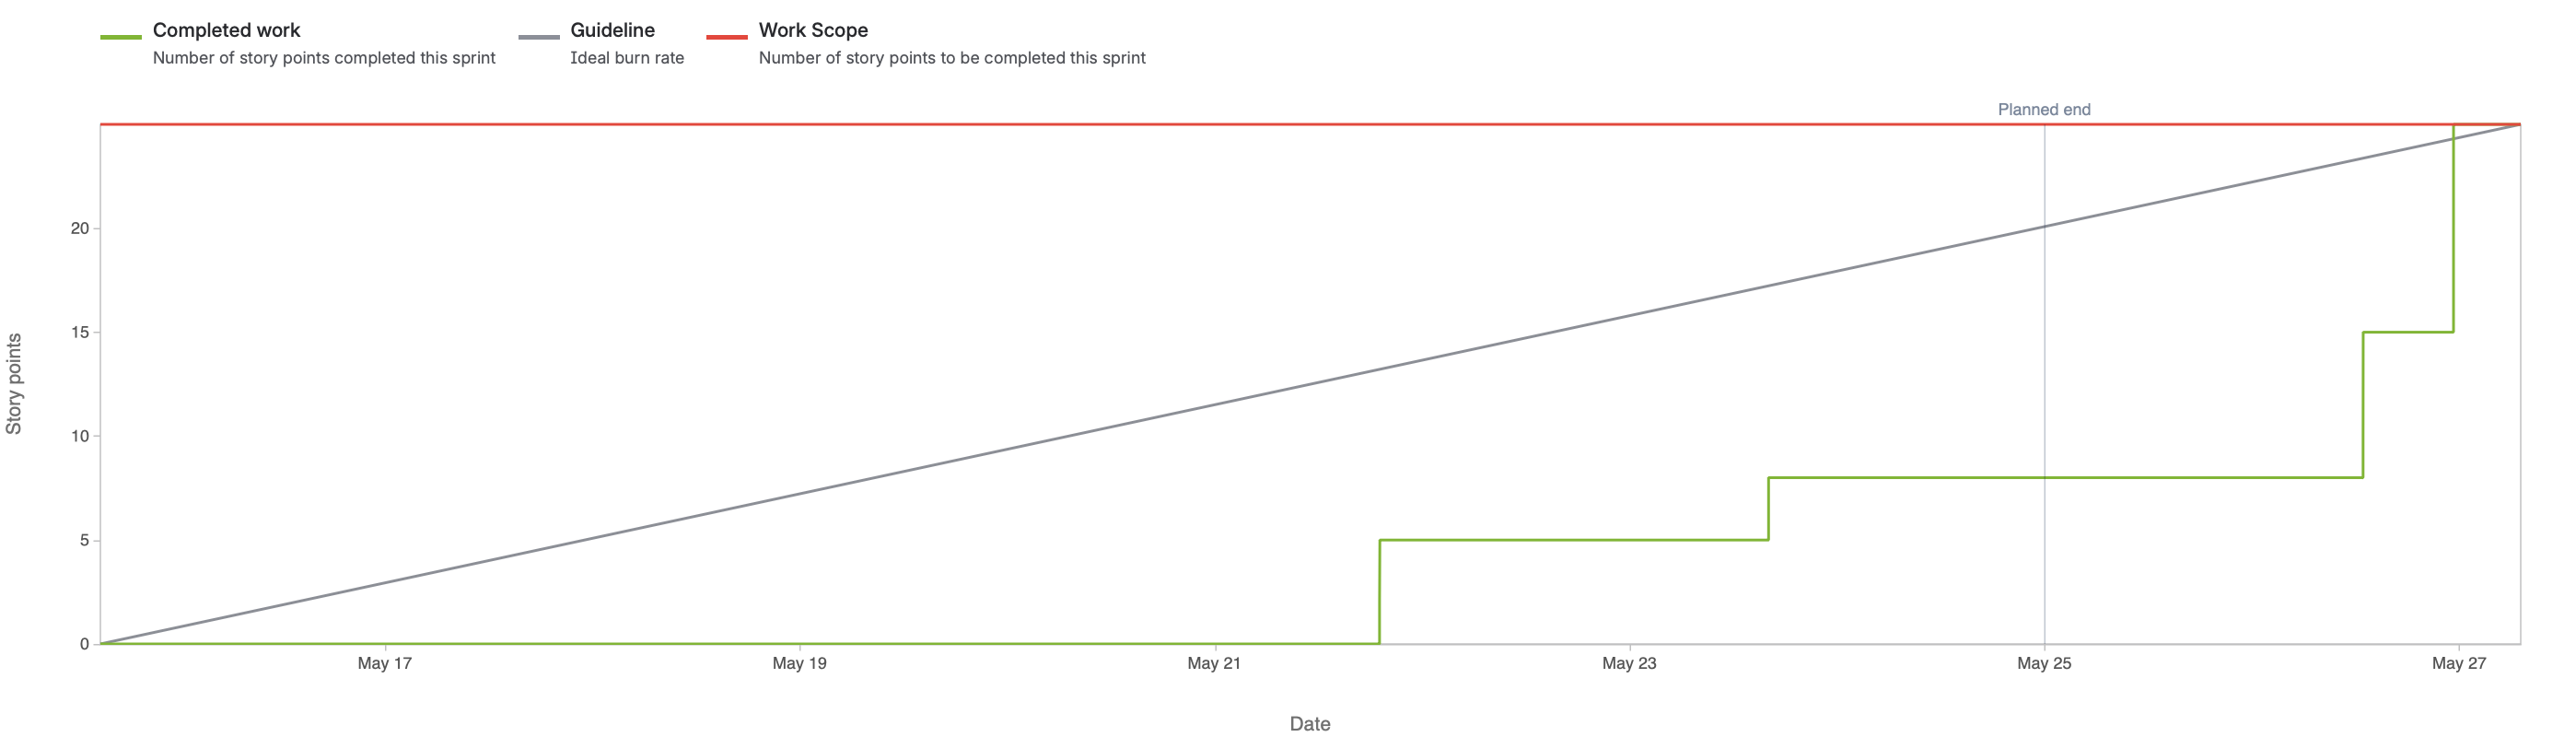
\includegraphics[width=0.8\linewidth,height=\textheight,keepaspectratio]{assets/sprints/sprint2-burndown.png}
\caption{Sprint 2 burndown chart.}\label{fig:sprint2-burndown}
\end{figure}

\begin{figure}
\centering
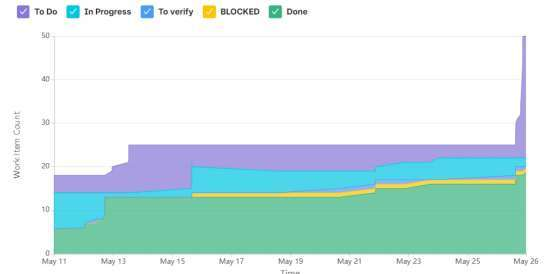
\includegraphics[width=0.62\linewidth,height=\textheight,keepaspectratio]{assets/sprints/sprint2-cumulative-flow.jpg}
\caption{Sprint 2 cumulative flow diagram showing work item counts by status.}\label{fig:sprint2-cumulative-flow}
\end{figure}

\subsubsection{Sprint Retrospective}\label{sec:sprint2-retrospective}

The retrospective used a public Miro template adapted for a team of five, running an opening check-in with an impact and frequency mapping of sprint events, a targeted reflection on the two process concerns raised by the Sprint 1 reviewer, a visioning exercise for the next sprint, and a Circle of Influence step that sorted the outputs into what the team controls and what it can only influence. The in-person Interhyp meeting rated as the highest-impact positive event, while the absence of a literature basis for estimating complexity and recurring local model synchronization issues rated as the main friction points.

Two process problems were confirmed. The gap between the Tuesday and Thursday meetings proved too wide in the second half of the sprint, when dependencies between the larger tickets were highest, so an optional Friday stand-up was trialed. The three five-point tickets each hid several sub-deliverables that would have been more trackable as separate items, so the team agreed to split anything above three points at planning and to add a mid-sprint refinement session, a rule that visibly shaped the Sprint 3 backlog (\cref{sec:sprint3-planning}). The remaining actions were to reserve the end of the Tuesday session for pull request reviews, to use pair programming for large or high-risk tickets, and above all to integrate router, judge, and optimizer into a single end-to-end run.
